\section{Koncepcja proponowanego rozwiązania}

\qquad Algorytm klasyfikacji został podzielony na dwie części. W pierwszej następuje stworzenie obiektów przechowujących parametry niezbędnych wartości dla każdego z załamków QRS. Zakłada się jednocześnie, że wszystkie załamki zostały poprawnie wykryte przez poprzednie moduły. Dane wejściowe zostają znormalizowane i zkwantyzowane, następnie przeprowadzana jest procedura ekstrakcji cech. W drugiej części następuje klasyfikacja zespołów QRS. Polega on na  klasteryzacji każdego wykrytego zespołu QRS. Warto zaznaczyć, iż każdy współczynnik reprezentuje inną wielkość i z tego powodu wartość tolerancji jest dobierana dla każdego z nich indywidualnie. Do klasteryzacji wykorzystywany jest algorytm g-means clustering. Jego realizacją zajmują się klasy GMeans i SVMClassifier

\subsection{Poprzednie podrozdziały}

\subsection{Klasyfikacja}

\qquad Aby sklasyfikować powstałe w poprzednim kroku klastry wykorzystano klasyfikator SVM (Support Vector Machine). W najprostszej postaci klasyfikator ten służy do wyznaczenia hiperpłaszczyzny rozdzielającej dwa liniowo separowalne zbiory. Hiperpłaszczyzna ta wyznaczana jest z maksymalnym marginesem, tzn. tak, aby suma jej odległości od najbliższych próbek z obu klas była jak największa (patrz rys. \ref{fig:SVM}).

\begin{figure}[h]
	\centering
	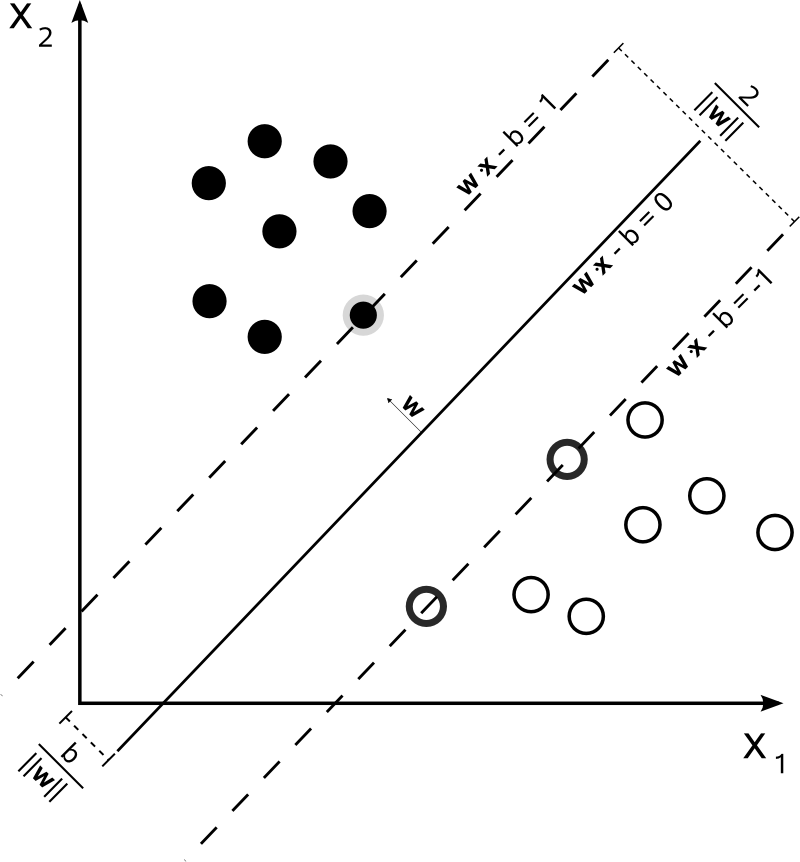
\includegraphics[width=8cm]{Grafika/Svm_max_sep_hyperplane_with_margin}
	\caption{Dwuwymiarowy przypadek hiperpłaszczyzny rozdzielającej dwie klasy z zaznaczonym marginesem. Źródło \cite{SVMWiki}}
	\label{fig:SVM}
\end{figure}

\qquad W wielu przypadkach nie można zagwarantować liniowej separowalności zbiorów.  W takich sytuacjach stosuje się tzw. Kernel trick. Polega on na zwiększeniu wymiaru przestrzeni danych wejściowych, aby w nowej przestrzeni istniała własność liniowej separowalności zbiorów. W tym celu wykorzystuje się różne funkcje jądra (kernel functions). W opisywanym module wykorzystana została funkcja RBF (Radial Basis Function) określona wzorem:

\begin{equation}
\label{eq:RBF}
K(x,x') = \exp{\left(-\frac{{\|x-x'\|}^{2}}{2\sigma^2}\right)}
\end{equation}

\qquad Aby klasyfikator mógł działać wcześniej należy go wytrenować. Polega to na podaniu mu ciągu wektorów uczących. Opisywany klasyfikator został wytrenowany za pomocą bazy danych MIT-BIH Arrhythmia Database \cite{MITDB}. Gotowy model klasyfikatora wczytywany jest z pliku, w którym zapisane są różne parametry oraz zestaw wektorów nośnych, na których opiera się działanie metody SVM.
